%SourceDoc ../Spicer-Dissertation.Rnw
\chapter{Using R and SWeave within RStudio} 
\label{R and SWeave}

\section{Working with \LaTeX{} documents}
If you use \LaTeX{}, you may have discovered that various statistical packages like SAS, Stata and R have commands that will format output in  for you to cut and paste into your .tex file \cite{HelpStatPack}.   For example, the \texttt{xtable} command in R.  

With the SWeave package in RStudio you can put your code right in the document itself -- no cut and paste!  The code will execute and pass the output to your \LaTeX{} document.

% <<label=xtable_R,echo=FALSE,results=tex>>=
%  library (xtable)
%  data(tli)
%  fm2 <- lm(tlimth ~ sex*ethnicty, data=tli)
%  print(xtable(fm2, caption="Linear Model"), caption.placement="top") 
% @

% R setups
\section{Inserting R Code in the text}
\begin{wrapfigure}[8]{r}{0.4\textwidth}
  \vspace{-20pt}
  \begin{center}
    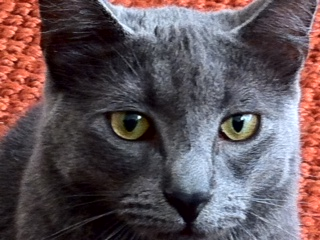
\includegraphics[width=0.38\textwidth]{esker.JPG}
  \end{center}
    \vspace{-20pt}
  \caption{Esker (a cat)}
\end{wrapfigure}
% Standard figure insertion without wrap
% \begin{figure}[h!] 
%     \centering
%    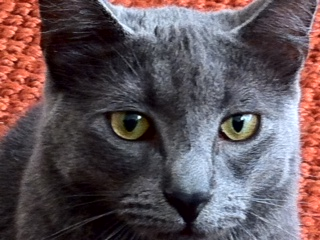
\includegraphics[width=3.0in]{esker.JPG}  
%      %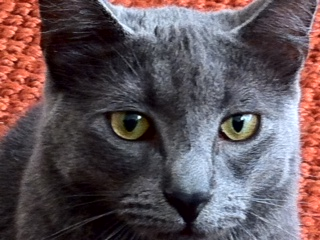
\includegraphics[width=3.0in]{esker} %if your use the \graphicspath command in the preamble.
%     \caption{Esker (aka, the cutest cat the world)}
%     \label{esker}
% \end{figure}

Consider the \texttt{cats} regression example from Venables \& Ripley
(1997) \cite{Venables:1997fk}. The data frame contains measurements of heart and body weight
of 144 cats (47 female,
97 male).The cats were all adult, over 2 kg body weight.   (To insert the number of cats into this paragraph, I just typed R code right into the paragraph itself using the \texttt{Sexpr} function.)


\section{Displaying R code and output}
A linear regression model of heart weight by body weight and gender was
fitted in R.  The R code for the model and the raw results that were sent to the R console can automatically appear within the document by specifying \texttt{echo=TRUE} (which is the default if you do not use the echo option)

\begin{Schunk}
\begin{Soutput}
Call:
lm(formula = Hwt ~ Bwt * Sex, data = cats)

Coefficients:
(Intercept)          Bwt         SexM     Bwt:SexM  
      2.981        2.636       -4.165        1.676  
\end{Soutput}
\end{Schunk}
\section{Using R functions that produce \texttt{tex}}
Tests for significance of the coefficients are shown in
Table~\ref{tab:coef}, a scatter plot including the regression lines is
shown in Figure~\ref{fig:cats}.  The table uses the \texttt{xtable} function, the R code chunk specifies the \texttt{results=tex} option to indicate that the output from the R code will already be formatted in \LaTeX{} and no further processing is necessary to compile the document.  SWeave will pull it in automagically.   Notice that \texttt{xtable} can insert a label that will be recognized in your document's List of Tables. 

% latex table generated in R 2.15.0 by xtable 1.7-0 package
% Fri Oct 12 08:59:12 2012
\begin{table}[ht]
\begin{center}
\begin{tabular}{rrrrr}
  \hline
 & Estimate & Std. Error & t value & Pr($>$$|$t$|$) \\ 
  \hline
(Intercept) & 2.9813 & 1.8428 & 1.62 & 0.1080 \\ 
  Bwt & 2.6364 & 0.7759 & 3.40 & 0.0009 \\ 
  SexM & -4.1654 & 2.0618 & -2.02 & 0.0453 \\ 
  Bwt:SexM & 1.6763 & 0.8373 & 2.00 & 0.0472 \\ 
   \hline
\end{tabular}
\caption{Linear regression model for cats data.}
\label{tab:coef}
\end{center}
\end{table}
\section{Including graphics}
The \texttt{echo=FALSE} option was used to suppress the display of the R code that produced the figure.  Notice that the caption and label are created using \LaTeX{} rather than within R.  This allows for the figure to be referenced in the List of Figures at the beginning of the document. 

\begin{figure}[h]
\begin{center}
\includegraphics{Chapter-1-004}
  \caption{The cats data from package MASS.}
  \label{fig:cats}
\end{center}  
\end{figure}

\section{Chunks}

When you compile your document to PDF the R code will run, but you will notice that it does \textbf{not} run in your current workspace.  If you are still debugging your code you will want to be able to view the objects and dataframes and see output in the console.   You can execute the code as though it was in a stand-alone R script by using the `Chunks' menu.

\section{A few \LaTeX{} tips}

To type equation in Latex, use the equation environment.

\begin{equation}
     \label{simple_equation}
 L' = {L}{\sqrt{1-\frac{v^2}{c^2}}}
\end{equation}

If you want your formula (or elements of a formula) to appear in the line of a text. Use a single \$ to begin and end the formula, such as \label{sympi} $\pi = 3.14$

A more sophisticated example using the double \$ does not number the formula:
$$SD_{wy} = \sqrt{\dfrac{\sum(y_i-\bar{y}{_w})^2 w_i}{\sum w_i -1}}$$

Of course with R you can use what you know about \LaTeX{} equations to insert math directly in your plot. In this code chunk the title is a fixed equation but the $\bar(x),\bar(y)$ axis labels will be dynamically constructed as the code is evaluated.

\begin{figure}[h]
\begin{center}
\begin{Schunk}
\begin{Sinput}
> x <- rnorm(100)
> y <- x + rnorm(100, sd = 0.5)
> plot(x, y,
+      xlab=substitute(bar(x) == k, list(k=mean(x))),
+      ylab=substitute(bar(y) == k, list(k=mean(y))),
+      main = expression("The mean (" * bar(x) * ") is " *
+                      sum(x[i]/n,i==1,n))
+      )
\end{Sinput}
\end{Schunk}
\includegraphics{Chapter-1-005}
  \caption{Plotting with Math.}
  \label{fig:mathplot}
\end{center}
\end{figure}
